\documentclass[12pt]{article}

\usepackage[utf8]{inputenc}
\usepackage{amsmath, amssymb}
\usepackage{geometry}
\usepackage{tikz}
\usetikzlibrary{arrows.meta}

\geometry{margin=1in}
\setlength{\parindent}{0pt}

\title{Solutions--In-Class Exercise}
\author{ECON 300 -- Labour Economics}
\date{Winter 2026}

\begin{document}
\maketitle
\hrule



\vspace{1em}

\section*{Common Setup (Reminders)}

Total time: \(T=80\). Leisure \(L\) on horizontal axis, consumption \(C\) on vertical axis.\\
Hours worked: \(h = 80 - L\). Wage: \(w = 20\).

\textbf{Baseline (no demogrant):}
\[
C = 20h = 20(80-L) = 1600 - 20L.
\]
So the baseline budget line:
\begin{itemize}
\item passes through \((L=80, C=0)\) (no work),
\item passes through \((L=0, C=1600)\) (work 80 hours),
\item has slope \(-w = -20\).
\end{itemize}

\section*{Key labour-supply logic (what to look for in answers)}

\begin{itemize}
\item \textbf{Income effect:} More non-labour income (or higher transfer) raises feasible consumption; if leisure is normal, tends to \(\uparrow L\) (less work).
\item \textbf{Substitution effect:} Any policy that reduces the effective net wage (flatter budget line) makes leisure cheaper relative to consumption; tends to \(\uparrow L\) (less work). If net wage increases, substitution effect tends to \(\downarrow L\) (more work).
\item \textbf{Participation (extensive margin):} Policies that raise consumption specifically at \(h=0\) or create large kinks/jumps around \(h=0\) often have the largest participation response.
\item \textbf{Reservation wage:} The minimum wage needed to make working (even a little) preferable to not working. Policies that make \(h=0\) more attractive tend to \(\uparrow w^R\).
\end{itemize}

\newpage

\section*{Policy A: Universal Lump-Sum Demogrant}

\textbf{Policy:} Everyone receives \$400 regardless of work.
\[
C = 400 + 20h = 400 + 1600 - 20L = 2000 - 20L.
\]

\subsection*{Diagram (Policy A vs Baseline)}

\begin{center}
\begin{tikzpicture}[x=0.09cm,y=0.0048cm]
  % Axes
  \draw[->,thick] (0,0) -- (95,0) node[below] {Leisure $L$ (hours)};
  \draw[->,thick] (0,0) -- (0,2200) node[left] {Consumption $C$ (\$)};

  % Ticks
  \foreach \x/\lab in {0/0,60/60,80/80} \draw (\x,0) -- (\x,-50) node[below] {\lab};
  \foreach \y/\lab in {0/0,400/400,1600/1600,2000/2000} \draw (0,\y) -- (-2,\y) node[left] {\lab};

  % Baseline line: from (80,0) to (0,1600)
  \draw[thick] (80,0) -- (0,1600) node[pos=0.55,above right] {Baseline};

  % Policy A line: from (80,400) to (0,2000)
  \draw[thick,dashed] (80,400) -- (0,2000) node[pos=0.55,above right] {Policy A};

  % Points
  \fill (80,0) circle (18);
  \fill (80,400) circle (18);

  \node[below right] at (80,0) {\small $(80,0)$};
  \node[above right] at (80,400) {\small $(80,400)$};
\end{tikzpicture}
\end{center}

\subsection*{Answer Key (Policy A)}

\begin{enumerate}
\item \textbf{Budget constraint change:} A \textbf{parallel upward shift} by \$400. Same slope \(-20\).
\item \textbf{Substitution effect?} \textbf{No.} The slope (net wage) is unchanged.
\item \textbf{Income effect:} \textbf{Yes.} Higher non-labour income makes the person richer; if leisure is normal, they choose \(\uparrow L\) (less work).
\item \textbf{Predictions:}
\begin{itemize}
\item \textbf{Hours worked:} typically \(\downarrow h\) (pure income effect).
\item \textbf{Participation:} may fall for marginal participants (those close to indifference at \(h=0\)), but generally the strongest effect is on \emph{hours}, not necessarily a large discrete participation jump.
\end{itemize}
\end{enumerate}

\newpage

\section*{Policy B: Targeted Demogrant (Non-Workers Only)}

\textbf{Policy:} \$400 only if \(h=0\).
\[
C =
\begin{cases}
400 & \text{if } h=0 \ (L=80),\\
20h = 1600-20L & \text{if } h>0 \ (L<80).
\end{cases}
\]

\subsection*{Diagram (discontinuity at $h=0$ / $L=80$)}

\begin{center}
\begin{tikzpicture}[x=0.09cm,y=0.0048cm]
  % Axes
  \draw[->,thick] (0,0) -- (95,0) node[below] {Leisure $L$ (hours)};
  \draw[->,thick] (0,0) -- (0,2000) node[left] {Consumption $C$ (\$)};

  % Ticks
  \foreach \x/\lab in {0/0,60/60,80/80} \draw (\x,0) -- (\x,-50) node[below] {\lab};
  \foreach \y/\lab in {0/0,400/400,1600/1600} \draw (0,\y) -- (-2,\y) node[left] {\lab};

  % Baseline/work line (applies for L<80)
  \draw[thick] (80,0) -- (0,1600) node[pos=0.55,above right] {Work region ($h>0$)};

  % Open circle at (80,0) (not attainable if must have h>0 to be on line)
  \draw[thick,fill=white] (80,0) circle (20);

  % Filled point at (80,400) for non-work benefit
  \fill (80,400) circle (18);
  \node[above right] at (80,400) {\small Demogrant at $h=0$};

  % Label
  \node[below right] at (80,0) {\small $(80,0)$ open};
  \node[above right] at (80,400) {\small $(80,400)$};
\end{tikzpicture}
\end{center}

\subsection*{Answer Key (Policy B)}

\begin{enumerate}
\item \textbf{Budget set shape:} Same baseline line for \(h>0\), plus a \textbf{jump up} to a higher point at \(h=0\) (a discontinuity at \(L=80\)).
\item \textbf{Reservation wage:} \textbf{Increases.} The outside option (\(h=0\)) is now better, so a higher wage is needed to induce participation for marginal workers.
\item \textbf{Which margin is most affected?} \textbf{Participation (extensive margin).} The policy directly rewards non-work, creating a strong incentive to choose \(h=0\).
\item \textbf{Prediction:} More people choose \(h=0\) (non-participation), especially those with high value of leisure or low market wages.
\end{enumerate}

\textbf{Instructor note (common misconception):} Students may call this a ``pure income effect.'' It is \emph{not} just income: the design creates a discontinuity that changes the work/non-work choice sharply (a strong extensive-margin distortion).

\newpage

\section*{Policy C: Phased-Out Demogrant (Negative Income Tax Style)}

\textbf{Policy:} \$400, phased out at 50\% of earnings. Net-of-benefit-reduction wage is lower.
\[
C = 400 + (1-0.5)\cdot 20h = 400 + 10h.
\]
In terms of leisure:
\[
C = 400 + 10(80-L) = 1200 - 10L.
\]

\subsection*{Diagram (flatter budget line: lower net wage)}

\begin{center}
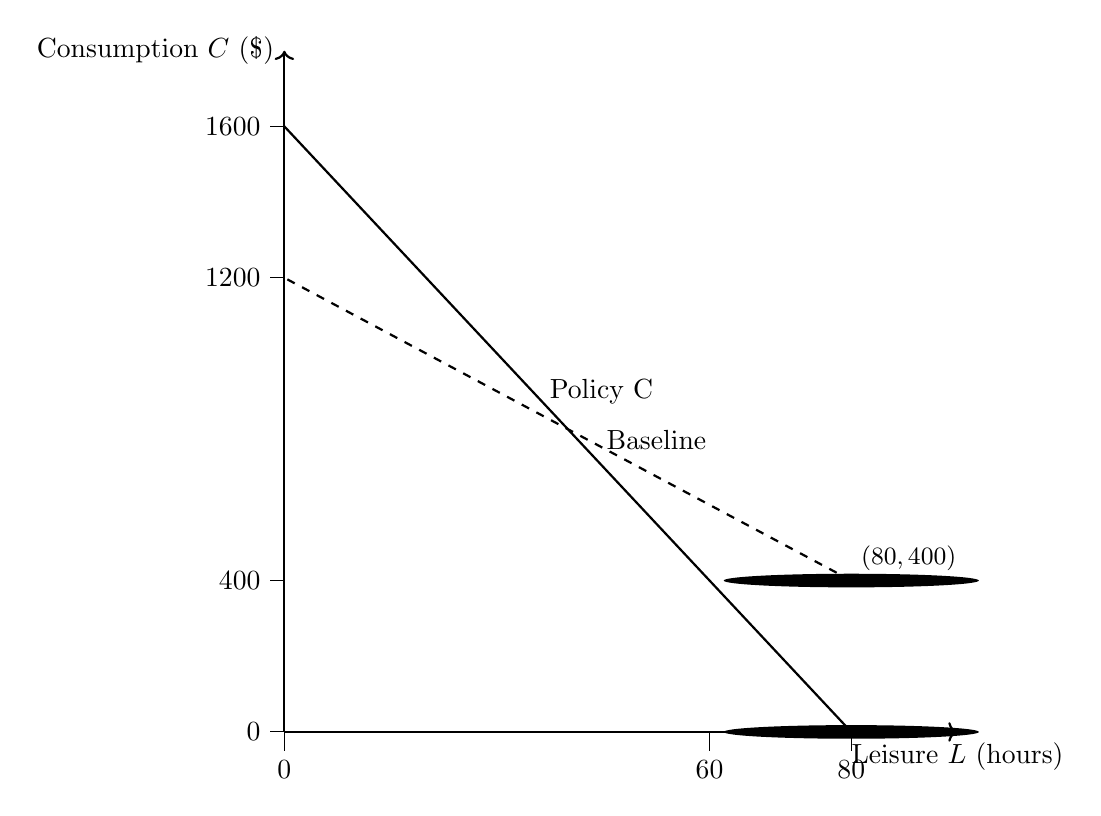
\begin{tikzpicture}[x=0.09cm,y=0.0048cm]
  % Axes
  \draw[->,thick] (0,0) -- (95,0) node[below] {Leisure $L$ (hours)};
  \draw[->,thick] (0,0) -- (0,1800) node[left] {Consumption $C$ (\$)};

  % Ticks
  \foreach \x/\lab in {0/0,60/60,80/80} \draw (\x,0) -- (\x,-50) node[below] {\lab};
  \foreach \y/\lab in {0/0,400/400,1200/1200,1600/1600} \draw (0,\y) -- (-2,\y) node[left] {\lab};

  % Baseline line
  \draw[thick] (80,0) -- (0,1600) node[pos=0.45,above right] {Baseline};

  % Policy C line: from (80,400) to (0,1200)
  \draw[thick,dashed] (80,400) -- (0,1200) node[pos=0.55,above right] {Policy C};

  % Points
  \fill (80,0) circle (18);
  \fill (80,400) circle (18);
  \node[above right] at (80,400) {\small $(80,400)$};
\end{tikzpicture}
\end{center}

\subsection*{Answer Key (Policy C)}

\begin{enumerate}
\item \textbf{Slope comparison:} Baseline slope is \(-20\). Policy C slope is \(-10\) (flatter). This reflects a lower \textbf{net wage} due to benefit phase-out.
\item \textbf{Income effect:} \textbf{Yes} (transfer increases non-labour income at any given \(h\), especially near \(h=0\)).
\item \textbf{Substitution effect:} \textbf{Yes} because the net wage falls from 20 to 10; leisure becomes cheaper relative to consumption, encouraging \(\uparrow L\) (less work).
\item \textbf{Predictions:}
\begin{itemize}
\item \textbf{Hours conditional on working:} tends to \(\downarrow h\) (both income and substitution reduce work).
\item \textbf{Participation:} also tends to fall for marginal workers (better outside option + weaker reward to working an extra hour).
\end{itemize}
\end{enumerate}

\textbf{Instructor note:} This is the classic case where you should expect stronger labour supply reductions than Policy A because Policy A has no substitution effect.

\newpage

\section*{Policy D: Conditional Demogrant (Work Requirement)}

\textbf{Policy:} \$400 only if \(h\ge 20\) (equivalently \(L \le 60\)).
\[
C =
\begin{cases}
20h = 1600-20L & \text{if } h<20 \ (L>60),\\
400 + 20h = 2000-20L & \text{if } h\ge 20 \ (L\le 60).
\end{cases}
\]
At the threshold \(h=20\) (\(L=60\)):
\[
C_{\text{below}} = 20\cdot 20 = 400,\qquad
C_{\text{eligible}} = 400 + 20\cdot 20 = 800.
\]
So there is a \textbf{jump of \$400} at \(L=60\).

\subsection*{Diagram (jump at eligibility threshold $h=20$ / $L=60$)}

\begin{center}
\begin{tikzpicture}[x=0.09cm,y=0.0048cm]
  % Axes
  \draw[->,thick] (0,0) -- (95,0) node[below] {Leisure $L$ (hours)};
  \draw[->,thick] (0,0) -- (0,2200) node[left] {Consumption $C$ (\$)};

  % Ticks
  \foreach \x/\lab in {0/0,60/60,80/80} \draw (\x,0) -- (\x,-50) node[below] {\lab};
  \foreach \y/\lab in {0/0,400/400,800/800,1600/1600,2000/2000} \draw (0,\y) -- (-2,\y) node[left] {\lab};

  % Baseline segment (ineligible region): L in (60,80]
  \draw[thick] (80,0) -- (60,400) node[pos=0.55,above right] {Ineligible ($h<20$)};

  % Eligible segment: parallel up by 400 for L in [0,60]
  \draw[thick,dashed] (60,800) -- (0,2000) node[pos=0.55,above right] {Eligible ($h\ge 20$)};

  % Threshold markers
  \draw[dotted,thick] (60,0) -- (60,900);
  \node[below] at (60,0) {\small threshold};

  % Open circle at ineligible point (60,400)
  \draw[thick,fill=white] (60,400) circle (20);

  % Filled circle at eligible point (60,800)
  \fill (60,800) circle (18);

  \node[right] at (60,400) {\small $(60,400)$ open};
  \node[right] at (60,800) {\small $(60,800)$};
\end{tikzpicture}
\end{center}

\subsection*{Answer Key (Policy D)}

\begin{enumerate}
\item \textbf{Budget set shape:} Baseline applies for \(h<20\). At \(h=20\) there is a \textbf{discrete jump up} in consumption, then the eligible region is a parallel upward shift (same slope \(-20\)).
\item \textbf{Effect near 20 hours:} Strong incentive to work at least 20 hours to ``qualify'' for the lump-sum payment.
\item \textbf{Distortion created:} A \textbf{notch} / eligibility discontinuity at \(h=20\) (or \(L=60\)), which can cause \textbf{bunching} (clustering) just at/above 20 hours.
\item \textbf{Predictions:}
\begin{itemize}
\item Some individuals who would have chosen slightly less than 20 hours may increase hours to reach eligibility (participation may increase for some, or hours may jump).
\item Individuals already above 20 hours experience a pure income effect (may reduce hours slightly while staying eligible).
\item Overall, expect \textbf{clustering at the threshold} and non-smooth labour supply responses.
\end{itemize}
\end{enumerate}

\section*{Wrap-Up Discussion: Suggested Answers}

\begin{enumerate}
\item \textbf{Only income effect:} Policy A (universal lump sum, no change in slope).\\
\textbf{Income + substitution effects:} Policy C (phase-out reduces net wage, flattening budget line).\\
\textbf{Discontinuity-driven extensive-margin distortion:} Policy B and Policy D.
\item \textbf{Most likely to reduce participation:} Policy B (pays only if not working).\\
\textbf{Most likely to reduce hours among workers:} Policy C (lower net wage + transfer).\\
Policy A tends to reduce hours via income effect; participation effect depends on how close people are to the margin.
\item \textbf{Why governments use conditional/phased-out designs:} targeting fiscal resources to low-income households, political preferences for ``work incentives,'' and budget constraints; but these designs often create stronger behavioural distortions (kinks/notches, reduced net wage).
\end{enumerate}

\end{document}
